\problem{}

1. Analyze the time complexities of the following algorithms and explain your reasoning.

\begin{algorithm}
\caption{}
\begin{algorithmic}
\For{$i \gets 1$ \textbf{to} $n$ \textbf{by} $i \gets 2i$}
    \For{$j \gets n$ \textbf{downto} $0$ \textbf{by} $j \gets j / 2$}
        \For{$k \gets j$ \textbf{to} $n$ \textbf{by} $k \gets k + 2$}
            \State $res \gets res + ij + jk$
        \EndFor
    \EndFor
\EndFor
\end{algorithmic}
\end{algorithm}


\begin{algorithm}
\caption{}
\begin{algorithmic}
\For{$i \gets n$ \textbf{downto} $0$}
    \For{$j \gets 1$ \textbf{to} $n$ \textbf{by} $j \gets 2j$}
        \For{$k \gets 0$ \textbf{to} $j$}
            \State $res \gets res + ij + jk$
        \EndFor
    \EndFor
\EndFor
\end{algorithmic}
\end{algorithm}

\noindent 2. Solve the following recurrence relations. Do not use the Master Theorem. Show all of your work.
$$T(n) = T(n-k) + 2k$$
$$T(n) = 2^kT(n/2^k) + kn$$
$$T(n) = 2^kT(n/2^k) + 2^k-1$$


\solution{}

1. (1)Algorithm 1:\\
The $i$-th loop runs $\log_{2}{n}$ times.\\
Suppose $n=2^x$, i.e. $x=\log_{2}{n}$, then for the $j$-th loop and the $k$-th loop, the total computation is:
$$\dfrac{1}{2}(2^x-0)+\sum_{j=0}^{x}\dfrac{1}{2}(2^x-2^j)=2^{x-1}+\dfrac{1}{2}(x+1)2^x-\dfrac{1}{2}(2^{x+1}-1)=O(x2^x)=O(n\log n)$$
Combine the $i$-th loop, the computation is
$$\log n\cdot O(n\log n)=O(n\log^2 n)$$
So above all, the total time complexity is $O(n\log_2^2{n})$.\\

(2) Algorithm 2:\\
The $i$-th loop runs $n+1$ times.\\
Suppose $n=2^x$, i.e. $x=\log_{2}{n}$, then for the $j$-th loop and the $k$-th loop, the total computation is:
$$\sum_{j=0}^{x}(2^j+1)=(2^{x+1}-1)+(x+1)=O(2^x)=O(n)$$
Combine the $i$-th loop, the computation is
$$(n+1)\cdot O(n)=O(n^2)$$
So above all, the total time complexity is $O(n^2)$.\\

2. (1) Suppose $n=c\cdot k$, i.e. $c=\dfrac{n}{k}$, then we have
\begin{align*}
    T(ck) &= T[(c-1)k]+2k\\
    T[(c-1)k] &= T[(c-2)k]+2k\\
    &\cdots\\
    T(2k) &= T(k)+2k\\
    T(k) &= T(0)+2k\\
\end{align*}
And all these equations, we have
$$T(ck)=T(0)+c\cdot (2k)=O\left(\dfrac{n}{k}\cdot 2k\right)=O(n)$$
So above all, $T(n)=O(n)$.\\

\begin{figure}[htbp]
    \centering
    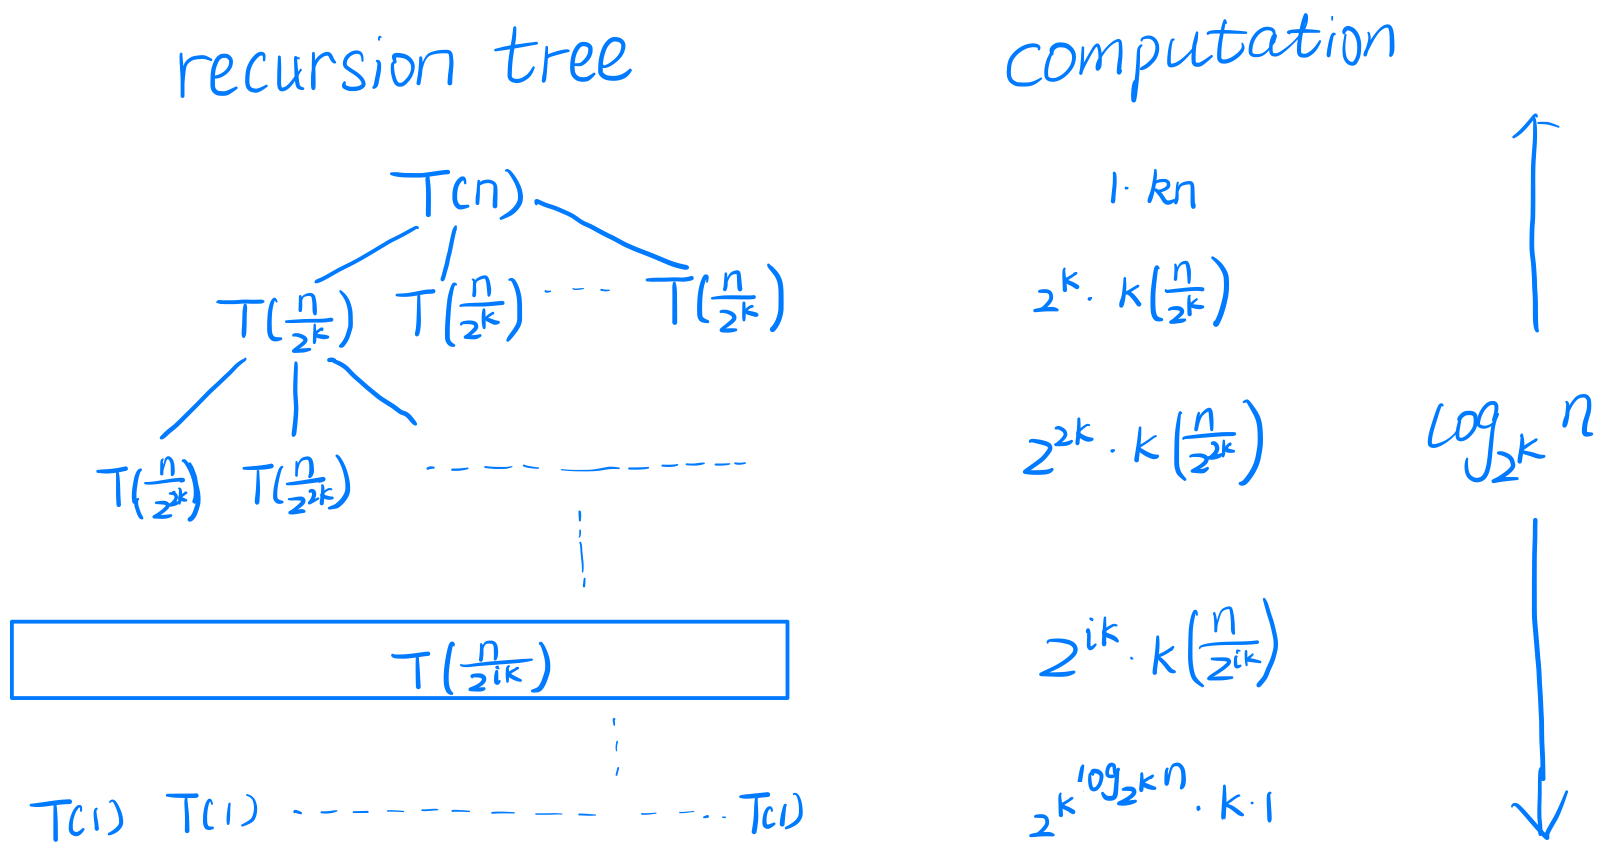
\includegraphics[width=\linewidth]{./figure/t1_22.png}
    \caption{The recursion tree of $T(n) = 2^kT(n/2^k) + kn$}
    \label{fig:t1_22}
\end{figure}

(2) From the recursion tree Figure \ref{fig:t1_22}, we can get that the total computation is:
\begin{align*}
    T(n) &= \sum_{i=0}^{\log_{(2^k)}{n}}(2^k)^i\cdot k\cdot\dfrac{n}{(2^k)^i}\\
         &= \sum_{i=0}^{\frac{1}{k}\log_{2}{n}} kn\\
         &= O((\dfrac{1}{k}\log_{2}{n})\cdot kn)\\
         &= O(n\log{n})
\end{align*}
So above all, $T(n)=O(n\log n)$.\\

\begin{figure}[htbp]
    \centering
    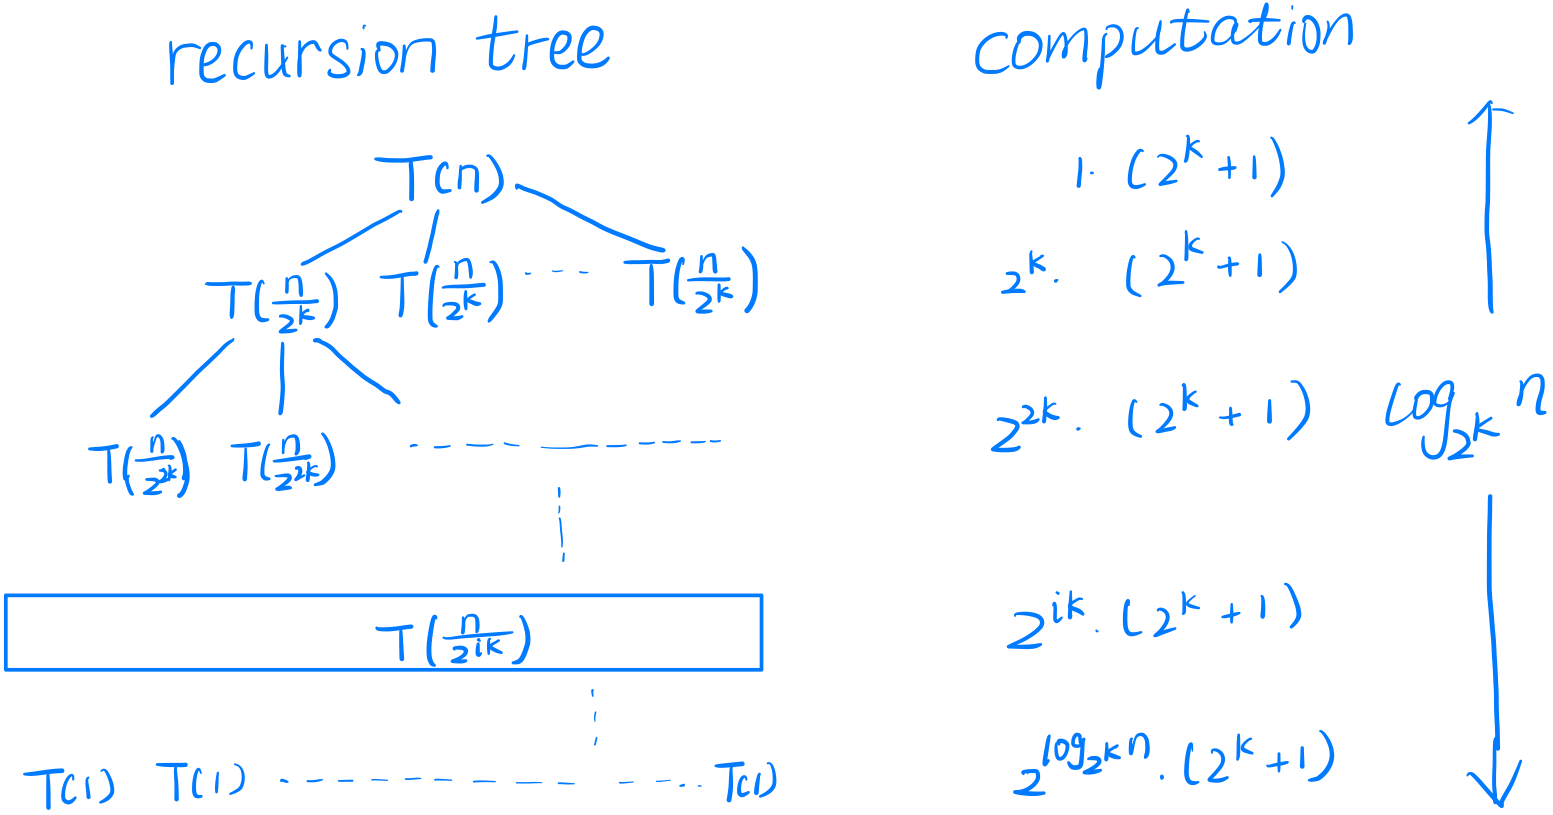
\includegraphics[width=\linewidth]{./figure/t1_23.png}
    \caption{The recursion tree of $T(n) = 2^kT(n/2^k) + 2^k-1$}
    \label{fig:t1_23}
\end{figure}

(3) Similarly with (2), from the recursion tree Figure \ref{fig:t1_23}, we can get that the total computation is:

\begin{align*}
    T(n) &= \sum_{i=0}^{\log_{(2^k)}{n}}(2^k)^i\cdot (2^k-1)\\
         &= O((2^k-1)\cdot \dfrac{(2^k)^{\frac{1}{k}\log_{2}{n}}-1}{2^k-1})\\
         &= O(n)
\end{align*}
So above all, $T(n)=O(n)$.\\



\newpage